\clearpage 

\section {Construction of Feldman-Cousins confidence regions}
\label{sec:fc}

The best-fit $|\Delta m^{2}_{23}|$ fluctuation seen in the analysis of the Run1 dataset is no longer present
(see Figs.\ \ref{fig:genie_deltachisq_dmsq_wide_3datasets} and \ref{fig:neut_deltachisq_dmsq_wide_3datasets}).
The analysis of the Run2 and the combined Run1+2 datasets strongly disfavours any interpretation of the 
observed 1 $\mu$-like ring event deficit in terms of large $|\Delta m^{2}_{23}|$ (a second or higher-order oscillation maximum 
at $\sim$600 MeV). Therefore, for reasons of {\em computational efficiency}, we limit the Feldman-Cousins
construction to the $|\Delta m^{2}_{23}|$ range from 1$\times$10$^{-3}$ $eV^{2}/c^{4}$ to 6$\times$10$^{-3}$ $eV^{2}/c^{4}$.

The application of the Feldman-Cousins method \cite{FeldmanCousins} to the T2K $\nu_{\mu}$-disappearance analysis
is discussed in detail in Sec. 3.4 of Ref. \cite{OurRun1DisappAnalysis}:
a number of toy MC experiment fits is performed for each point of the (sin$^{2}$2$\theta_{23}$, $|\Delta$m$^{2}_{23}|$)
2-dimensional grid.
For each grid point, the critical value of $\Delta\chi^{2}$ ($\Delta\chi^{2}_{critical}$)
is found such that $\alpha$ of the toy MC experiments have $\Delta\chi^{2}_{MC}$ $<$ $\Delta\chi^{2}_{critical}$,
where $\alpha$ is the desired confidence level (see Fig. \ref{fig:minos2011_dchisq_cumulative}).
The value of $\Delta\chi^{2}_{MC}$ for each toy MC experiment is calculated as follows:
\begin{equation}
\displaystyle
\Delta \chi^{2}_{MC} = \chi^{2} \textrm{(true)} - \chi^{2} \textrm{(MC, best-fit)}
\label{eq:deltachi2}
\end{equation}
where
``true'' means the true values of the oscillation parameters at that grid point, and
``best-fit'' means the best-fit values for that MC experiment (this is equivalent to 
equation 5.6 in \cite{FeldmanCousins}).
$\chi^{2}$ is defined as
\begin{equation}
\displaystyle
\chi^{2} (sin^{2}2\theta_{23},|\Delta m^{2}_{23}|;{\bf a}) =
  2 \cdot \sum_{i=0}^{N-1}
   \Big(
     n^{obs}_{i} \cdot ln(n^{obs}_{i}/n^{exp}_{i}) +
     (n^{exp}_{i}-n^{obs}_{i})
   \Big) 
\label{eq:chisquare}
\end{equation}
where
$N$ is the number of reconstructed energy bins,
${\bf a}$ is a vector of nuisance parameters (see Tab. \ref{tab:input_uncertainties}),
$n^{obs}_{i}$ is the observed number of events in the $i^{th}$ bin, and
$n^{exp}_{i} = n^{exp}_{i}(sin^{2}2\theta_{23},\Delta m^{2}_{23}; {\bf a})$
is the corresponding expected number of events. This definition of $\chi^{2}$ arises from our use
of the likelihood ratio method, which is explained in more detail in 
Sec.\ 3.2 of Ref.\ \cite{OurRun1DisappAnalysis}.

%In order to construct the Feldman-Cousins contour with statistical errors only 
%then only statistical fluctuations are in
%Different values of $\Delta\chi^{2}_{critical}$ are calculated for th
%are unchanged and they are described in
%Sections 3.1, 3.2 and 
%As in Ref. \cite{OurRun1DisappAnalysis}, systematic errors were included in the oscillation contours
%using the Cousins and Highland method (Bayesian integration) and by determining their effect on the
%Feldman and Cousins $\Delta\chi^{2}_{critical}$ values.

\begin{figure*}[htb]
\center
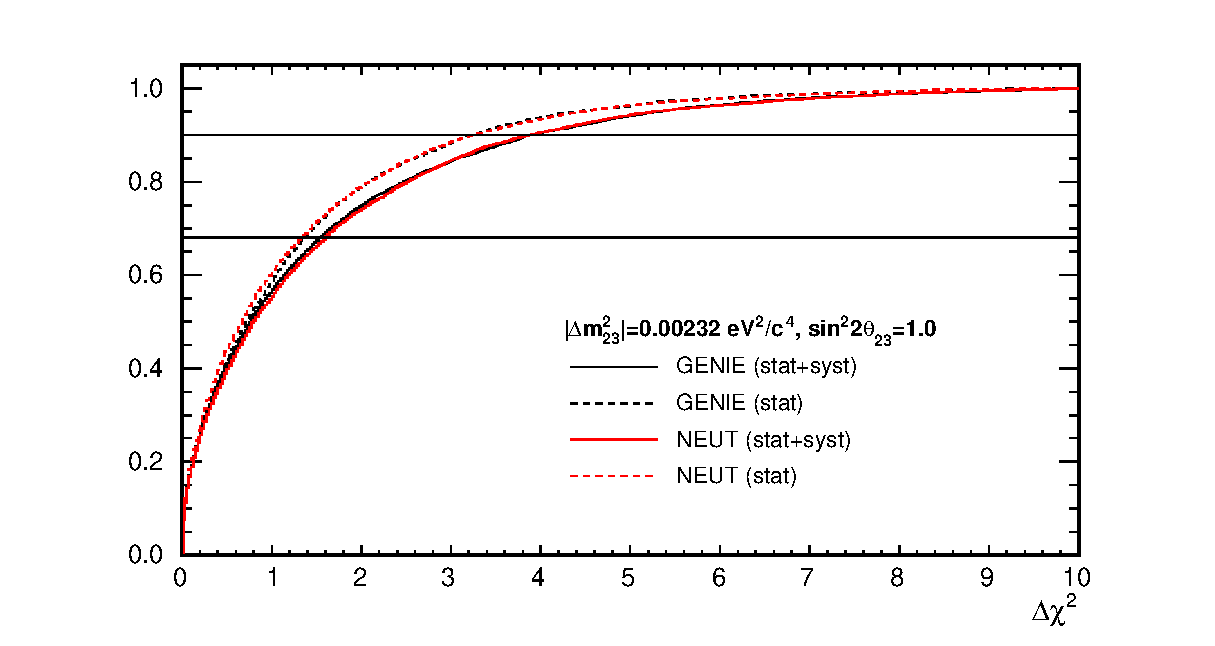
\includegraphics[width=40pc]{./images/feldman_cousins/minos2011_dchisq_cummulative.eps}
\caption{
  Cumulative $\Delta\chi^{2}_{MC}$ distributions (for both NEUT and GENIE) for oscillated toy MC experiments generated
  with $sin^{2}2\theta_{23}$ = 1.0 and $|\Delta m^{2}_{23}|$ = 2.32$\times10^{-3}$ $eV^{2}/c^{4}$.
  The horizontal lines show the 68\% and 90\% levels
  (values of $\Delta\chi^{2}_{critical}$ are the values of $\Delta\chi^{2}_{MC}$ where these horizontal lines
  intersect with the cumulative distributions).
}
\label{fig:minos2011_dchisq_cumulative}
\end{figure*}

\begin{figure*}[htb]
\center
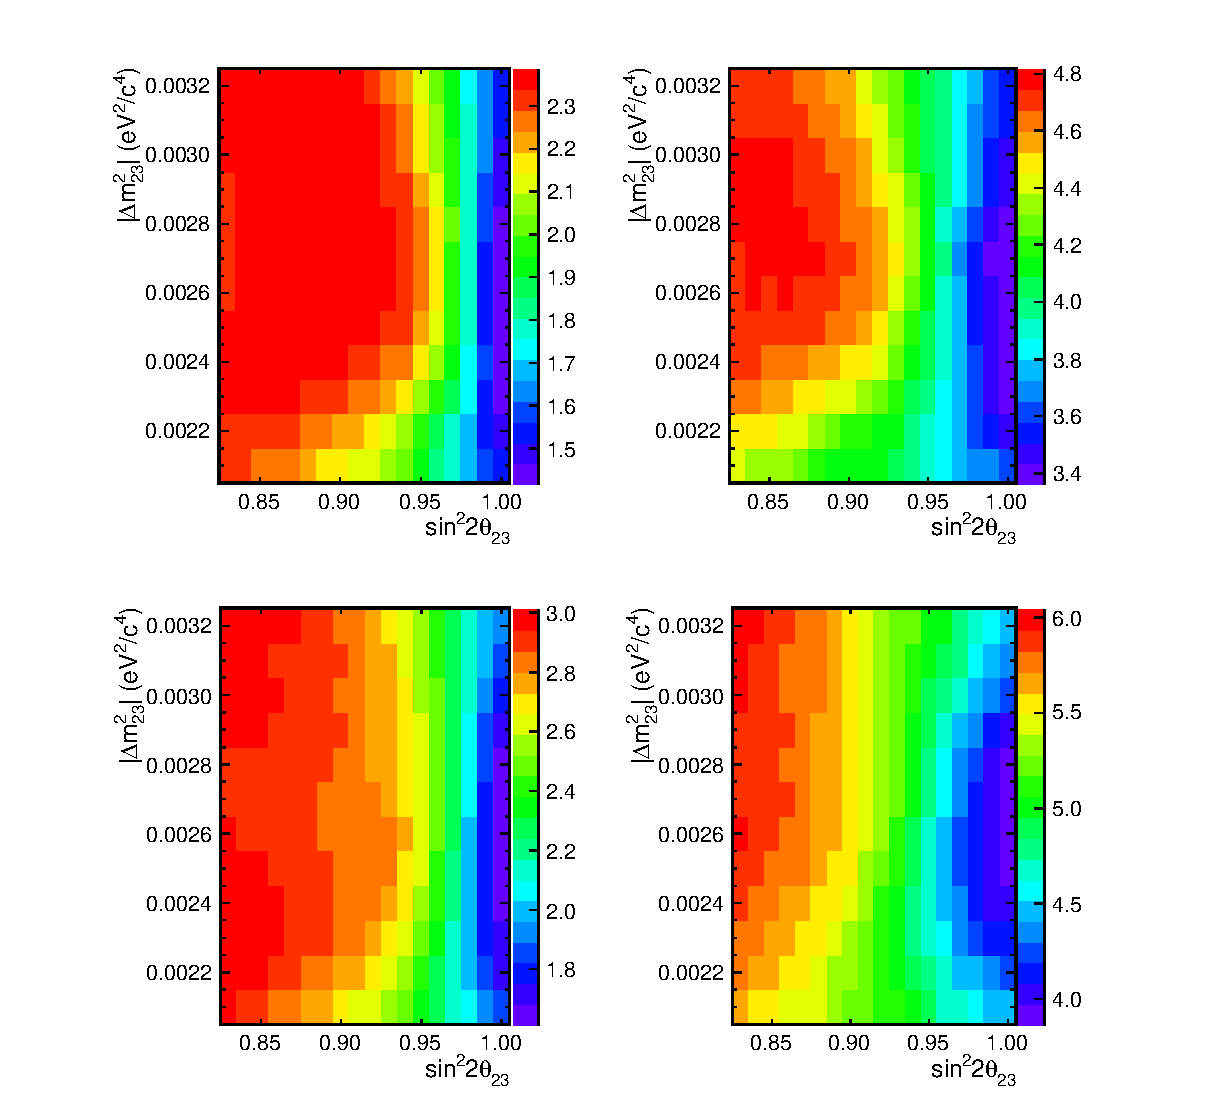
\includegraphics[width=38pc]{./images/feldman_cousins/fc_deltachisqcrit_2d_neut.eps}
\caption{
  Monte Carlo estimation (NEUT),
  according to the Feldman-Cousins method,
  of $\Delta\chi^{2}_{68}$ (left) and $\Delta\chi^{2}_{90}$ (right)
  as functions of $sin^{2}{2\theta_{23}}$ and $\Delta{m^{2}_{23}}$,
  for calculation of the 68\% (left) and 90\% (right) CL confidence regions
  for the $1.431 \times 10^{20}$-POT T2K 2-flavour $\nu_{\mu}$-disappearance analysis.
  The top row shows $\Delta\chi^{2}$ surfaces calculated using statistical fluctuations
  only whereas the bottom row shows $\Delta\chi^{2}$ surfaces calculated using
  both systematic variations and statistical fluctations.
  As expected from \cite{FeldmanCousins}, the values of $\Delta\chi^{2}$ 
  decrease as the
  physical boundary at $sin^{2}{2\theta_{23}}$ = 1 is approached. 
}
\label{fig:fc_deltachisqcrit_2d_neut}
\end{figure*}


\begin{figure*}[htb]
\center
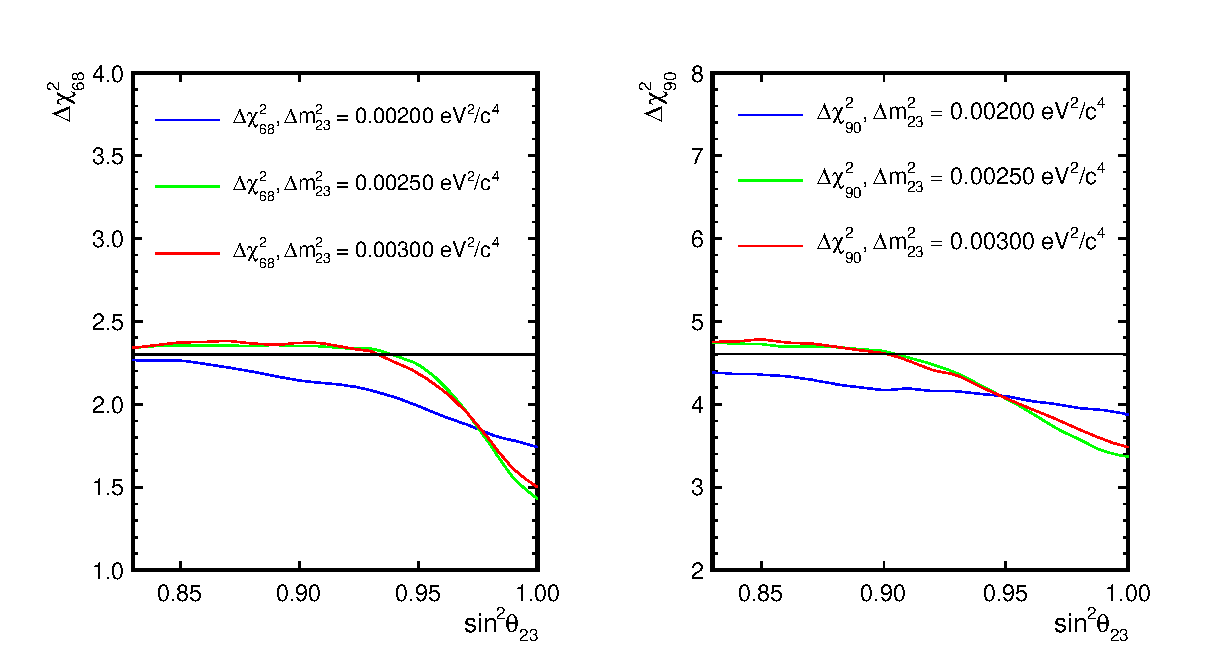
\includegraphics[width=38pc]{./images/feldman_cousins/fc_deltachisqcrit_statonly_vs_sinsq_3dmsq_neut.eps}
\caption{
  Monte Carlo estimation (NEUT),
  according to the Feldman-Cousins method (statistical errors only),
  of $\Delta\chi^{2}_{68}$ (left) and $\Delta\chi^{2}_{90}$ (right),
  as functions of $sin^{2}{2\theta_{23}}$ for 3 different values of $\Delta{m^{2}_{23}}$
  ($2.0 \times 10^{-3} eV^{2}/c^{4}$,
   $2.5 \times 10^{-3} eV^{2}/c^{4}$ and
   $3.0 \times 10^{-3} eV^{2}/c^{4}$).
  For comparison, the canonical value of $\Delta\chi^{2}$ used in the constant $\Delta\chi^{2}_{critical}$
  method is also shown as a horizontal line.
}
\label{fig:fc_deltachisqcrit_statonly_vs_sinsq_3dmsq_neut}
\end{figure*}

\begin{figure*}[htb]
\center
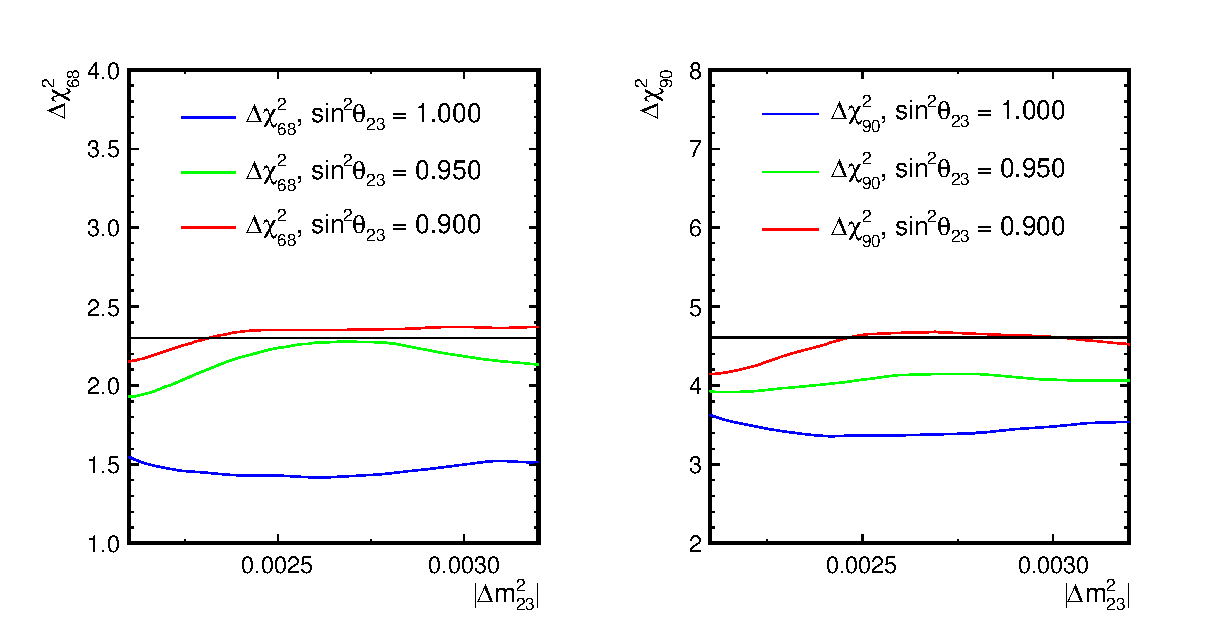
\includegraphics[width=38pc]{./images/feldman_cousins/fc_deltachisqcrit_statonly_vs_dmsq_3sinsq_neut.eps}
\caption{
  Monte Carlo estimation  (NEUT),
  according to the Feldman-Cousins method (statistical errors only),
  of $\Delta\chi^{2}_{68}$ (left) and $\Delta\chi^{2}_{90}$ (right),
  as functions of $\Delta{m^{2}_{23}}$ for 3 different values of $sin^{2}{2\theta_{23}}$
  (0.90, 0.95 and 1.00).
  For comparison, the canonical value of $\Delta\chi^{2}$ used in the constant $\Delta\chi^{2}_{critical}$
  method is also shown as a horizontal line.
}
\label{fig:fc_deltachisqcrit_statonly_vs_dmsq_3sinsq_neut}
\end{figure*}

